\chapter{Конструкторский раздел}
В данном разделе будут определены требования к программному обеспечению
и приведены схемы алгоритма полного перебора и муравьиного алгоритма для
решения задачи коммивояжера.

\section{Требования к программному обеспечению}
Входные данные: матрица стоимостей взвешенного неориентированного графа.

Выходные данные: кратчайший гамильтонов цикл.

\section{Представления алгоритмов}
На рисунках~\ref{fig:brute_force}~---~\ref{fig:ant} представлены схема алгоритма полного перебора и схема муравьиного алгоритма.

\begin{figure}[H]
    \centering
    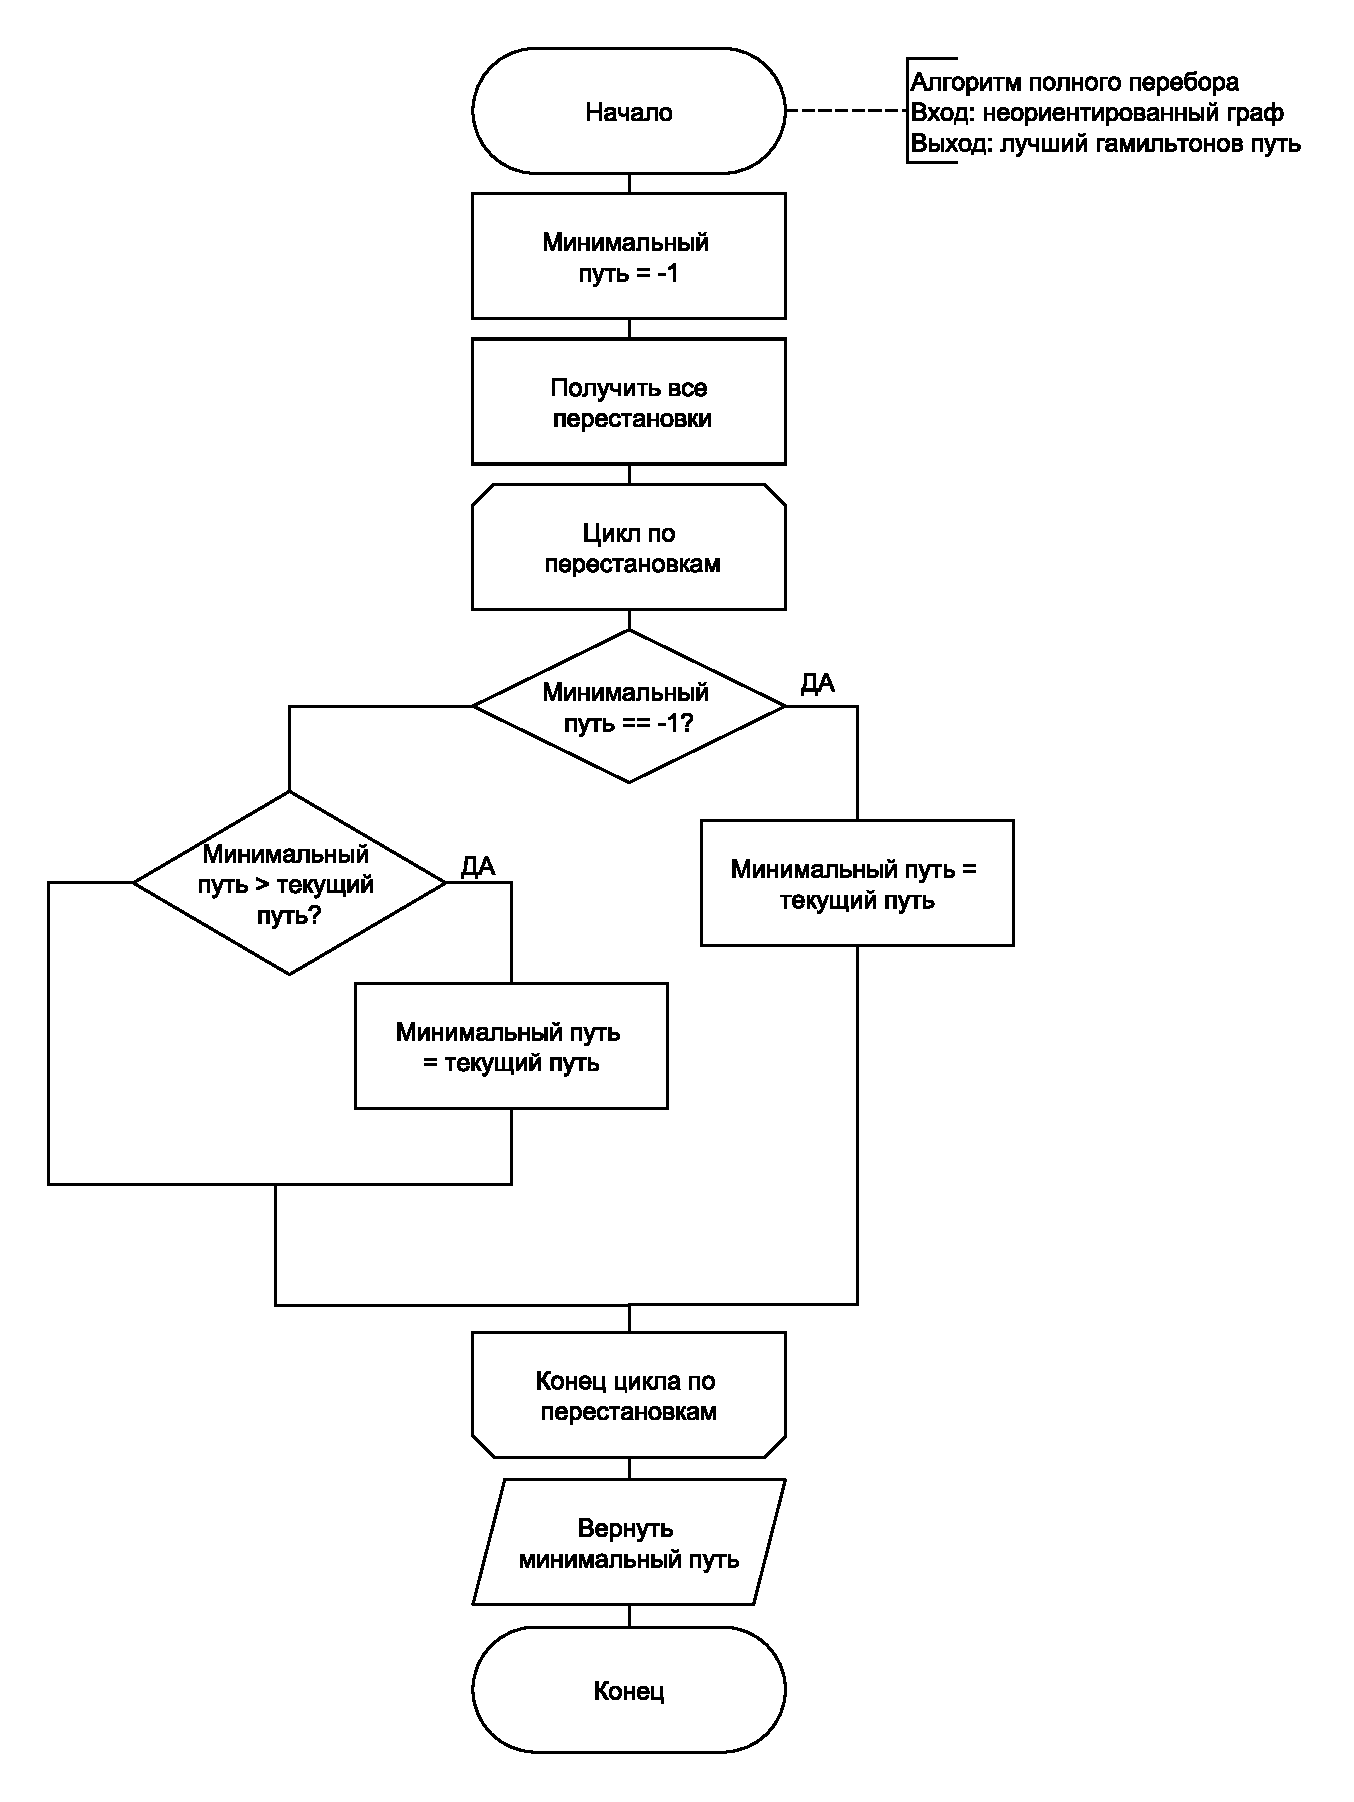
\includegraphics[scale=0.7]{img/unnamed1.eps}
    \caption{Схема алгоритма полного перебора}
    \label{fig:brute_force}
\end{figure}

\begin{figure}[H]
    \centering
    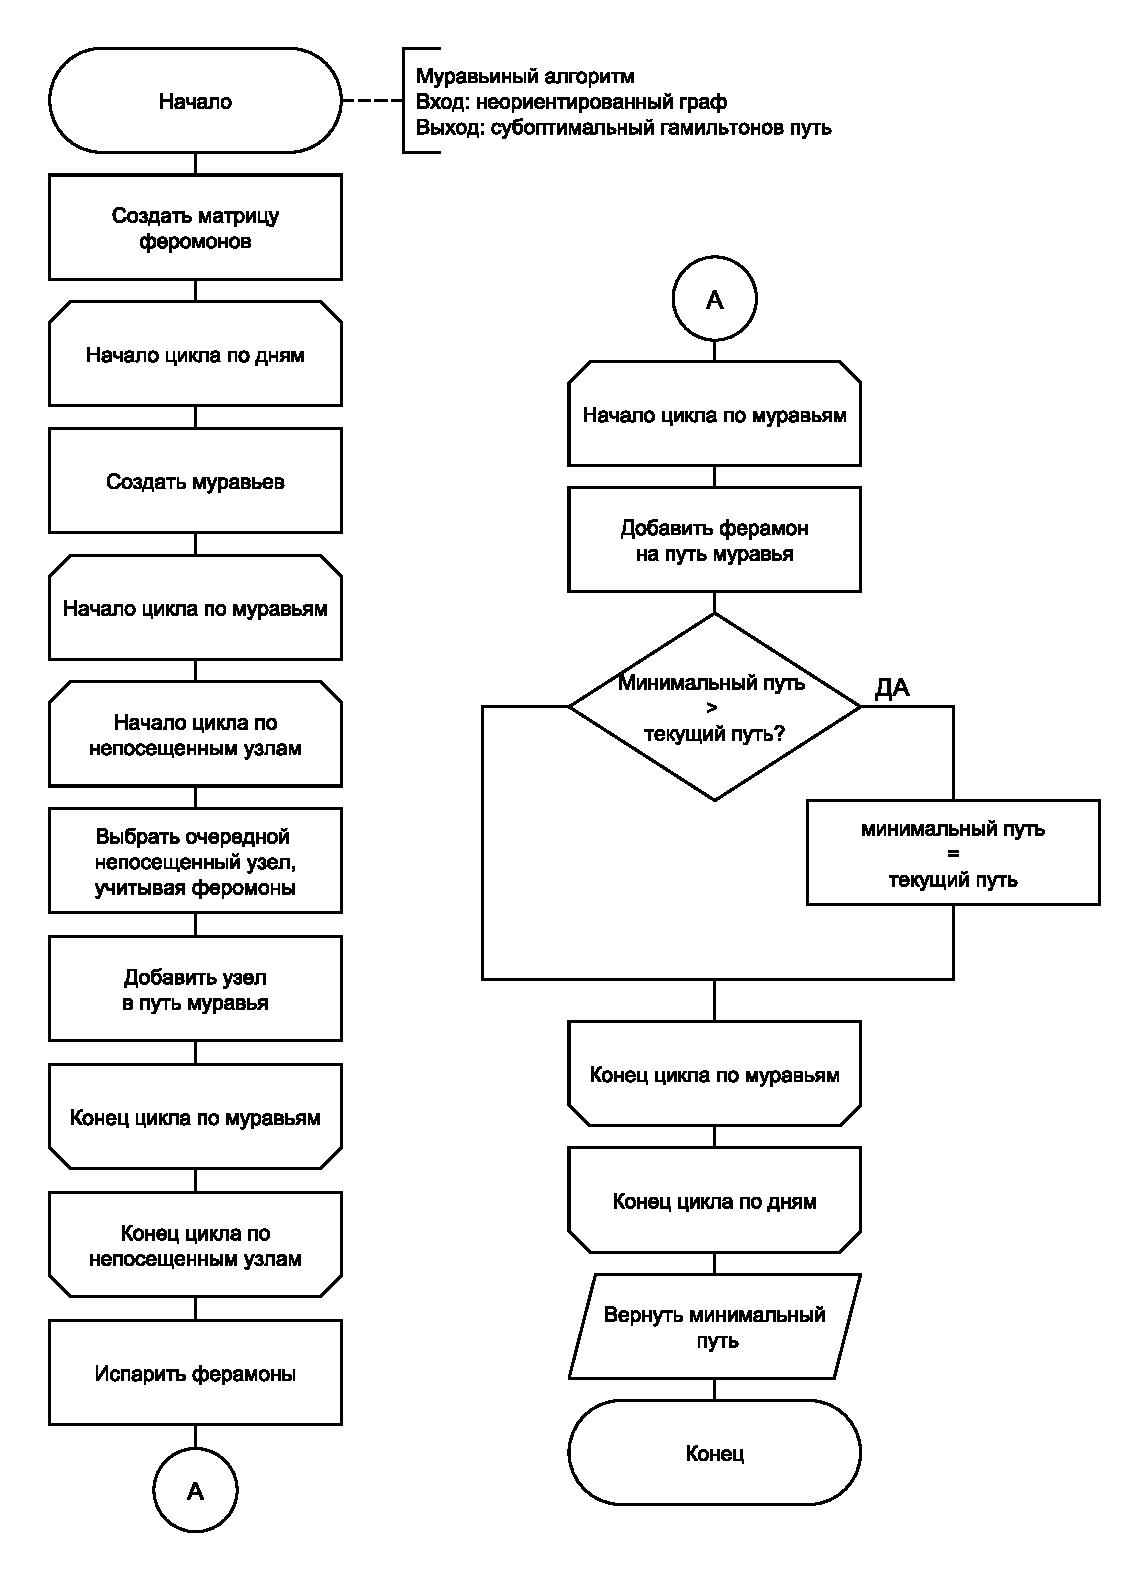
\includegraphics[scale=0.7]{img/unnamed2.eps}
    \caption{Схема муравьиного алгоритма}
    \label{fig:ant}
\end{figure}

\textbf{ВЫВОД}

В данном разделе были определены требования к программному обеспечению и приведены схемы алгоритмов полного перебора и муравьиного алгоритма для решения задачи коммивояжера.

\clearpage